\begin{figure}[htbp]
\centering
\begin{tikzpicture}[x=1cm,y=1cm]
\node[anchor=south west,inner sep=0] at (0,0) {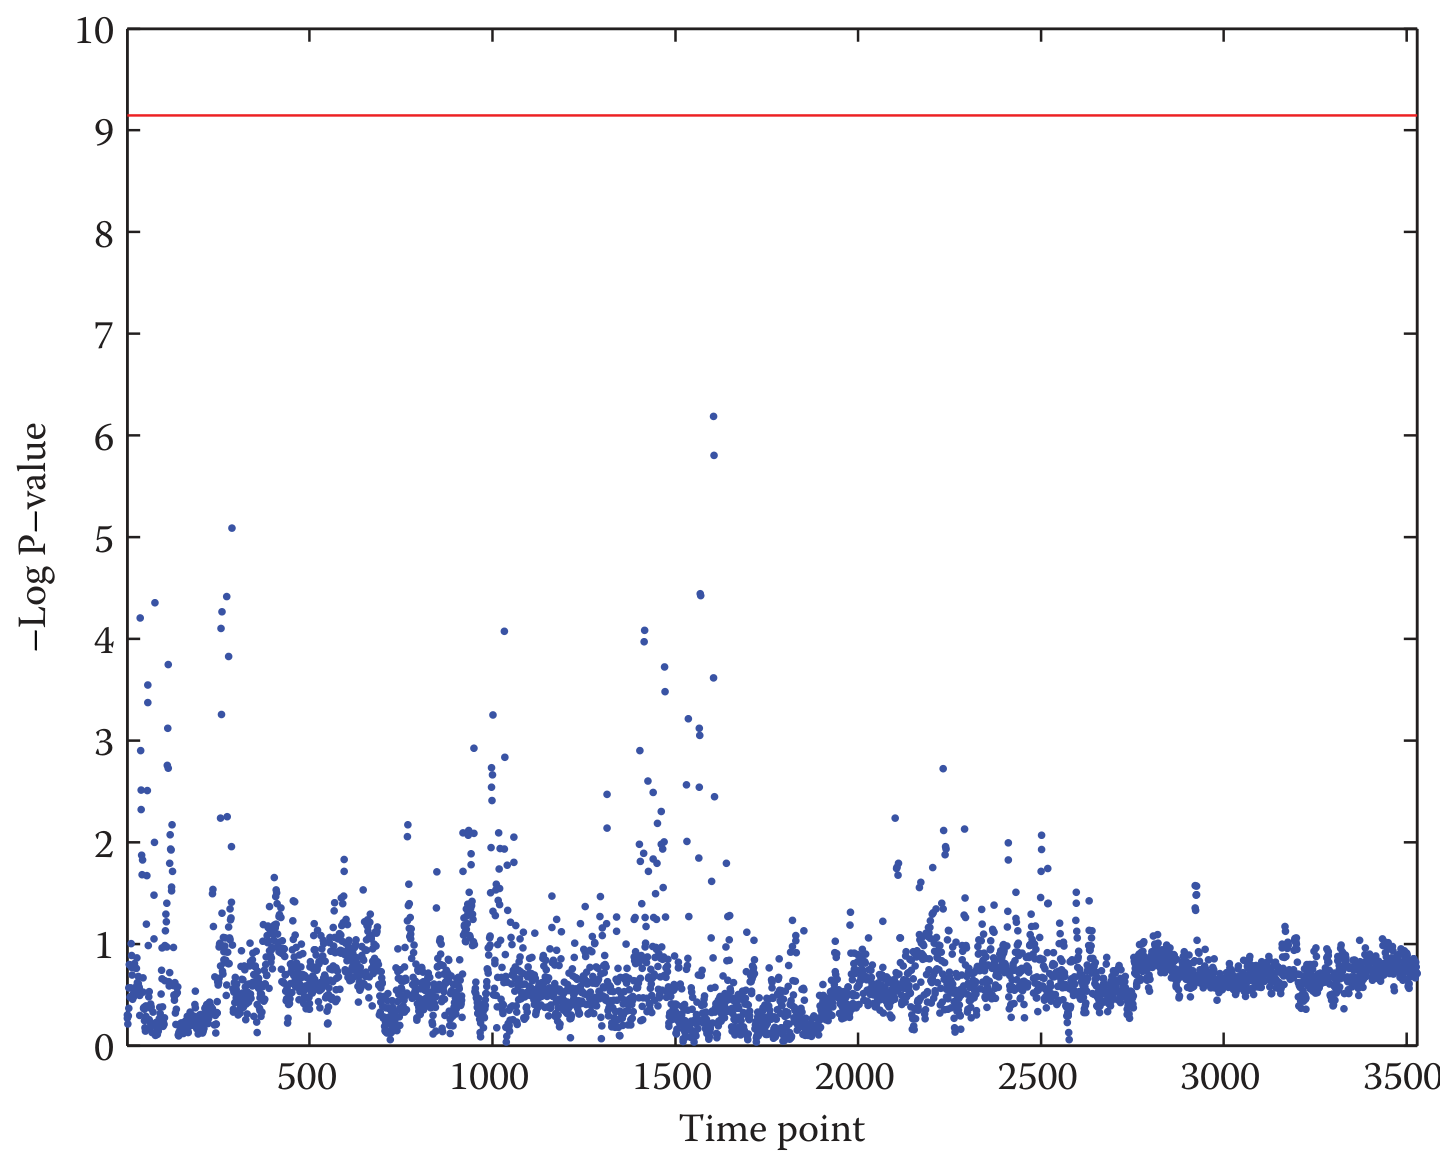
\includegraphics[width=13.8cm]{figures/ch03_fig20_data.png}};
\fill[white] (6.4679,0.0590) rectangle (8.3221,0.4903);
\node[font=\small,rotate=0,inner sep=0] at (7.3950,0.2747) {时间点};
\fill[white] (0.1155,4.8379) rectangle (0.5564,7.0934);
\node[font=\small,rotate=90,inner sep=0] at (0.3360,5.9656) {$-\log P$ 值};
\end{tikzpicture}
\origfig{20}{在各个时间点检验基因 ANKLE1 与血氧饱和度曲线关联所得的 $P$ 值。}
\label{fig:ch03-20}
\end{figure}
